\documentclass[12pt, twoside]{article}
\usepackage[letterpaper, margin=1in, head=30pt, headsep=0.1in]{geometry}
\usepackage[english]{babel}
\usepackage[utf8]{inputenc}
\usepackage{amsmath}
\usepackage{amsfonts}
\usepackage{amssymb}
\usepackage{tikz}
\usepackage{yhmath} %arcs using \wideparen{}
\usetikzlibrary{quotes, angles}

\usepackage{graphicx}
\usepackage{enumitem}
\usepackage{multicol}

%\usepackage{pgfplots}
%\pgfplotsset{width=10cm,compat=1.9}
%\usepgfplotslibrary{statistics}
%\usepackage{pgfplotstable}
%\usepackage{tkz-fct}
%\usepackage{venndiagram}

\usepackage{fancyhdr}
\pagestyle{fancy}
\fancyhf{}
\renewcommand{\headrulewidth}{0pt} % disable the underline of the header
\raggedbottom
\newif\ifmeta
\metatrue %print standards and topics tags

\title{High School Geometry problem sets}
\author{Chris Huson}
\date{April 2021}

%\fancyhead[RE]{\thepage}
%\fancyhead[RO]{\thepage \\ Name: \hspace{3cm}}
%\fancyhead[L]{BECA / Dr. Huson / 10th Grade Geometry\\* 7 June 2019}
%
%\begin{document}
%\subsubsection*{13.7 Homework: Cross sections, distance applications}
%\fancyhead[L]{BECA / Dr. Huson / Geometry 03-Volume+angle-bisectors\\* pset ID: 34}

\begin{document}

\subsubsection*{8.2 Sector calculations}
\begin{enumerate}
  \item Do Now: Convert each set of units. One inch $= \displaystyle \frac{1}{12}$ foot or one foot $= 12$ inches.
  \begin{enumerate}[itemsep=1.5cm]
    \item How many feet are 30 inches?
    \item How many inches are 8.25 feet?
  \end{enumerate}

\newpage
\item Do Now: The shaded sector of the unit circle is \emph{one tenth} of the whole circle, as shown.
  \begin{multicols}{2}
  \raggedcolumns
  \begin{enumerate}[itemsep=1.5cm]
    \item Write down the circumference in terms of $\pi$. ($C=2\pi r$)
    \item Find $m \angle AOB$ in \emph{degrees}.
    \item Find $m \angle AOB$ in \emph{radians}.
  \end{enumerate}
  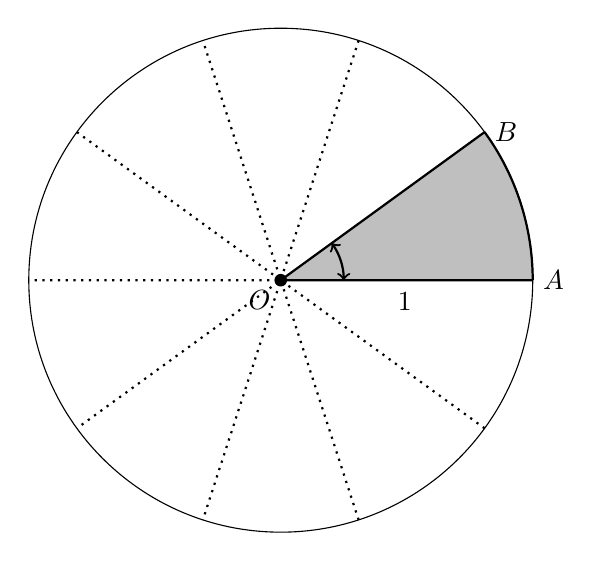
\begin{tikzpicture}[scale=0.8]
    \fill [lightgray]
    (0,0)--(0:4) arc (0:36:4)--(0,0);
    \draw (0,0) circle[radius=4];
    \draw [thick, <->] (0:1) arc (0:36:1);
    \draw [thick] (0:4) arc (0:36:4);
    \draw [thick]
    (0:4) node[right] {$A$}--
    (0,0) node[below left] {$O$}--
    (36:4) node[right] {$B$};
    \draw [thick, dotted](72:4)--(0,0)--(108:4);
    \draw [thick, dotted](144:4)--(0,0)--(180:4);
    \draw [thick, dotted](-72:4)--(0,0)--(-108:4);
    \draw [thick, dotted](-36:4)--(0,0)--(-144:4);
    \fill (0,0) circle[radius=.1];
    %\node at (18:4.5) {$?$};
    \node at (-10:2) {$1$};
  \end{tikzpicture}
  \end{multicols}

  \newpage
  \item Convert equivalent angle measures between \emph{radians} and \emph{degrees} ($2 \pi = 360^\circ$, $\pi = 180^\circ$).\\[0.25cm]
  Apply the appropriate formula.
  \begin{multicols}{2}
  $\displaystyle r = d \times \frac{\pi}{180}$\\
  $\displaystyle d = r \times \frac{180}{\pi}$
  \end{multicols}
    \begin{multicols}{2}
    \raggedcolumns
    \begin{enumerate}
      \item $72^\circ = \hspace{0.15cm} ?$ radians\\[0.5cm]
      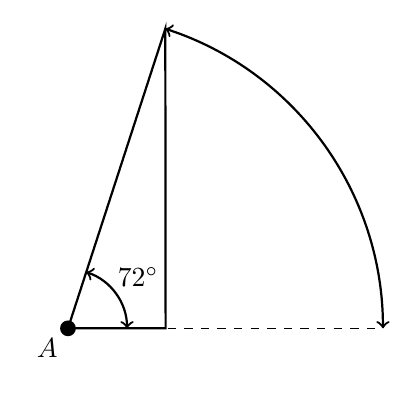
\begin{tikzpicture}[scale=1]
        \draw [thick, <->] (0:0.75) arc (0:72:0.75);
        \draw [thick, <->] (0:4) arc (0:72:4);
        \draw [dashed](0,0)--(4,0);
        \draw [thick]
        (0,0) node[below left] {$A$}--(72:4)--(1.24,0)--cycle;
        \fill (0,0) circle[radius=.1];
        \node at (36:1.1) {$72^\circ$};
      \end{tikzpicture}
      \item $\displaystyle \frac{\pi}{9}  = \hspace{0.15cm} ?$ degrees\\[0.75cm]
      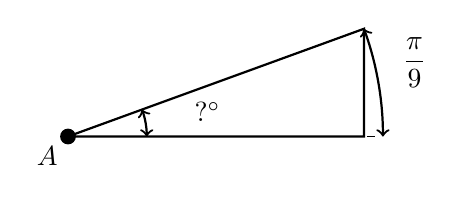
\begin{tikzpicture}[scale=1]
        \draw [thick, <->] (0:1) arc (0:20:1);
        \draw [thick, <->] (0:4) arc (0:20:4);
        \draw [dashed](0,0)--(4,0);
        \draw [thick]
        (0,0) node[below left] {$A$}--(20:4)--(3.76,0)--cycle;
        \fill (0,0) circle[radius=.1];
        \node at (10:1.8) {$?^\circ$};
        \node at (12:4.5) {$\displaystyle \frac{\pi}{9}$};
      \end{tikzpicture}
    \end{enumerate}
    \end{multicols}

\newpage
\item Groupwork: Each member picks a different color and Greek letter to write on other members' slides. 
\begin{enumerate}
  \item Hand write yours in the upper left quadrant first.
  \item In the breakout room, student with the shortest first name ``raises his/her hand'' and other members come to ``help'' him/her.
  \item Each student writes his/her name and letter into a different quadrant. (better: copy/paste screenshot)
  \item Repeat with each team member.
\end{enumerate}
\begin{center}
  \begin{tikzpicture}[scale=1, rotate=0]
  \draw [thick] (-5,0)--(5,0);
  \draw [thick] (0,-4)--(0,4);
  \node at (-4,4){Your letter:};
  \node at (3,4){Member name \& letter:};
  \node at (3,-0.5){Member name \& letter:};
  \node at (-4,-0.5){Member name \& letter:};
\end{tikzpicture}
\end{center}
Example Greek letters are 
{\Large$\pi$, $\theta$, $\alpha$, $\Delta$, $\beta$, $\sigma$, $\Sigma$, $\epsilon$ \par}

\newpage
\item Lesson: \emph{Pie charts} represent proportions using sector areas and central angles.
  \begin{multicols}{2}
  \raggedcolumns
  \begin{enumerate}%[itemsep=1.5cm]
    \item Population of NY City is 8,340,000\\
    Population of NY State is 19,500,000
    \item Find the fraction of New Yorkers, $x$, who reside in NYC as a percentage. \vspace{2cm}
    \item Find the central angle of the shaded area, $\theta = x \times 360^\circ$
  \end{enumerate}
  \columnbreak
  \begin{flushright}
    New York State
  \end{flushright}
  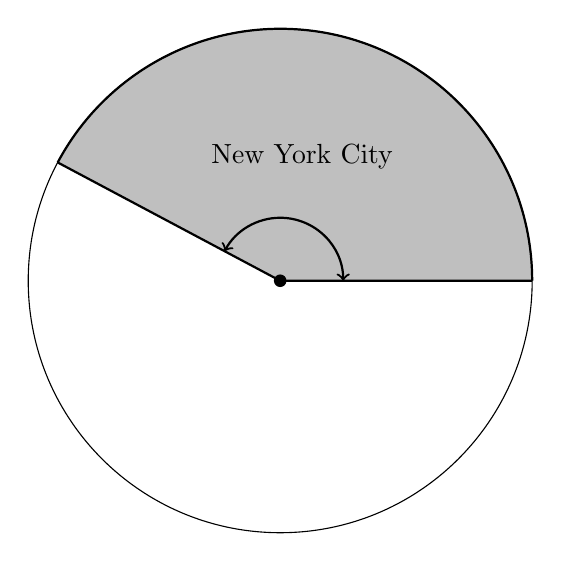
\begin{tikzpicture}[scale=0.8]
    \fill [lightgray]
    (0,0)--(0:4) arc (0:152:4)--(0,0);
    \draw (0,0) circle[radius=4];
    \draw [thick, <->] (0:1) arc (0:152:1);
    \draw [thick] (0:4) arc (0:152:4);
    \draw [thick]
    (0:4)--(0,0)--(152:4);
    %\draw [thick, dotted](72:4)--(0,0)--(108:4);
    %\draw [thick, dotted](144:4)--(0,0)--(180:4);
    %\draw [thick, dotted](-72:4)--(0,0)--(-108:4);
    %\draw [thick, dotted](-36:4)--(0,0)--(-144:4);
    \fill (0,0) circle[radius=.1];
    %\node at (18:4.5) {$?$};
    \node at (80:2) {New York City};
  \end{tikzpicture}
  \end{multicols}

\newpage
\item Practice: Convert between \emph{radians} to \emph{degrees} knowing $2 \pi = 360^\circ$ or $\pi = 180^\circ$.\\[0.25cm]
Apply the appropriate formula. Leave radians in terms of $\pi$.
\begin{multicols}{2}
$\displaystyle r = d \times \frac{\pi}{180}$\\
$\displaystyle d = r \times \frac{180}{\pi}$
\end{multicols}
  \begin{multicols}{2}
  \raggedcolumns
  \begin{enumerate}
    \item $36^\circ = \hspace{0.15cm} ?$ radians\\[0.5cm]
    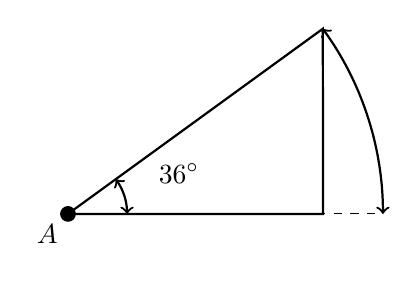
\begin{tikzpicture}[scale=1]
      \draw [thick, <->] (0:0.75) arc (0:36:0.75);
      \draw [thick, <->] (0:4) arc (0:36:4);
      \draw [dashed](0,0)--(4,0);
      \draw [thick]
      (0,0) node[below left] {$A$}--(36:4)--(3.24,0)--cycle;
      \fill (0,0) circle[radius=.1];
      \node at (20:1.5) {$36^\circ$};
    \end{tikzpicture}
    \item $72^\circ = \hspace{0.15cm} ?$ radians\\[0.5cm]
    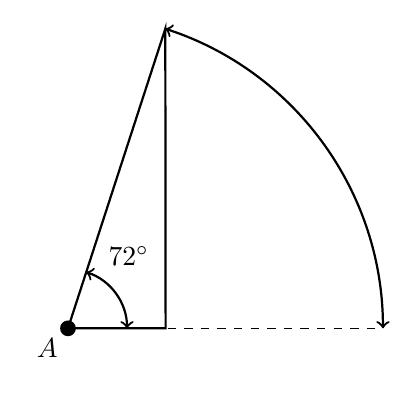
\begin{tikzpicture}[scale=1]
      \draw [thick, <->] (0:0.75) arc (0:72:0.75);
      \draw [thick, <->] (0:4) arc (0:72:4);
      \draw [dashed](0,0)--(4,0);
      \draw [thick]
      (0,0) node[below left] {$A$}--(72:4)--(1.24,0)--cycle;
      \fill (0,0) circle[radius=.1];
      \node at (50:1.2) {$72^\circ$};
    \end{tikzpicture}
    \item $\displaystyle \frac{\pi}{7}  = \hspace{0.15cm} ?$ degrees\\[0.5cm]
    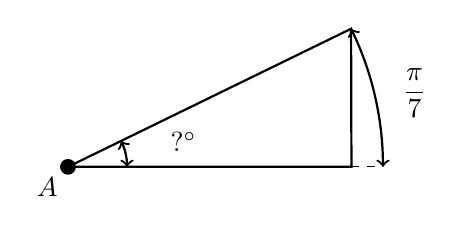
\begin{tikzpicture}[scale=1]
      \draw [thick, <->] (0:0.75) arc (0:26:0.75);
      \draw [thick, <->] (0:4) arc (0:26:4);
      \draw [dashed](0,0)--(4,0);
      \draw [thick]
      (0,0) node[below left] {$A$}--(26:4)--(3.6,0)--cycle;
      \fill (0,0) circle[radius=.1];
      \node at (12:1.5) {$?^\circ$};
      \node at (12:4.5) {$\displaystyle \frac{\pi}{7}$};
    \end{tikzpicture}
    \item $\displaystyle \frac{3\pi}{4}  = \hspace{0.15cm} ?$ degrees\\[0.75cm]
    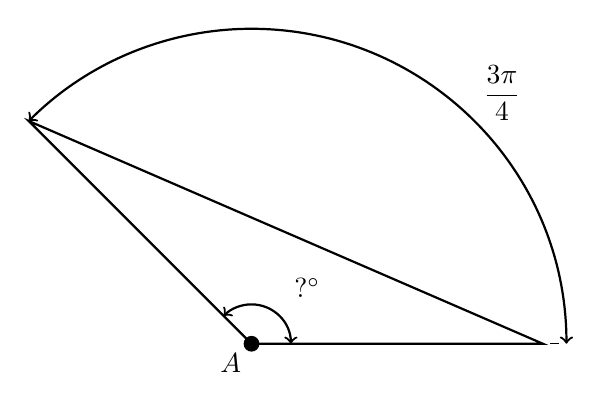
\begin{tikzpicture}[scale=1]
      \draw [thick, <->] (0:0.5) arc (0:135:0.5);
      \draw [thick, <->] (0:4) arc (0:135:4);
      \draw [dashed](0,0)--(4,0);
      \draw [thick]
      (0,0) node[below left] {$A$}--(135:4)--(3.7,0)--cycle;
      \fill (0,0) circle[radius=.1];
      \node at (45:1.) {$?^\circ$};
      \node at (45:4.5) {$\displaystyle \frac{3\pi}{4}$};
    \end{tikzpicture}
  \end{enumerate}
  \end{multicols}

\newpage
\item Right $\triangle ABC$ is drawn in \emph{standard position} with vertex $A$ on the origin and right $\angle C$ on the $x$-axis, as shown.
\begin{multicols}{2}
  \raggedcolumns
\begin{enumerate}
  \item Find the length of the hypotenuse $AB$ using the Pythagorean Theorem $a^2 + b^2 = c^2$. (leave as a radical)
  \vspace{3cm}
  \item Find the slope of the line segment $\overline{AB}$ as a decimal.
\end{enumerate}
  \begin{tikzpicture}[scale=0.7]
    %\draw [help lines] (-1.15,-1.2) grid (11,10);
    \draw [thick, ->] (-0.2,0) -- (9.4,0) node [above] {$x$};
    \foreach \x in {1,2,...,9}
      \draw[shift={(\x,0)},color=black] (0pt,2pt) -- (0pt,-2pt) node[below] {\footnotesize \; $\x$};
    \draw [thick, ->] (0,-0.2)--(0,9.6) node [left] {$y$};
    \foreach \y in {1,2,...,9}
      \draw[shift={(0,\y)},color=black] (-2pt,0pt) -- (2pt,0pt) node[left] {\footnotesize \; $\y$};
    \draw [-, thick] (0,0) node[below left] {$A$}
    --(5,0) node[above right] {$C$}
    --(5,4)node[right] {$B (5,4)$}--cycle;
    \draw (5,0)++ (-0.5,0)-- +(0,0.5)-- +(0.5,0.5);
    %\draw [<->, thick] (-0.6,4.3)--(5,8.5);
  \end{tikzpicture}
\end{multicols}


\end{enumerate}
\end{document}